\documentclass[10pt,twocolumn]{article}
\usepackage[margin=0.56in,top=0.60in,bottom=0.60in]{geometry}
\usepackage{amsmath,amssymb,amsthm}
\usepackage{booktabs}
\usepackage{graphicx}
\usepackage{microtype}
\usepackage[hidelinks]{hyperref}
\usepackage{xurl}

\raggedbottom
\setlength{\columnsep}{0.20in}
\setlength{\parskip}{1.5pt}
\setlength{\textfloatsep}{7pt plus 2pt minus 2pt}
\setlength{\dbltextfloatsep}{8pt plus 2pt minus 2pt}

\title{\vspace{-1.2em}\textbf{Exact Cyclotomic and Constructive Lean~4 Certificates for Symmetric Identities and Determinants of Legendre-Symbol Matrices}\vspace{-0.4em}}
\author{Lluis Eriksson\\
\small Independent Researcher (\nolinkurl{https://github.com/lluiseriksson})\\
\small Companion Preprint to Le~Lan--Liu (\texttt{arXiv:2611.33667v1}) --- Unrefereed Formal-Verification Artifact\vspace{-0.6em}}
\date{November 26, 2026}

\begin{document}
\maketitle

\begin{abstract}
\noindent Roman Le~Lan and Keqin Liu (\texttt{arXiv:2611.33667v1}, Nov.~2026) prove Zhi-Wei Sun's Conjecture~3.2(i), evaluating the four-parameter Legendre-symbol determinant $A(x,y,z,w) = \det\!\bigl[x + (\tfrac{i+j}{p}) + (\tfrac{i}{p})y + (\tfrac{j}{p})z + (\tfrac{ij}{p})w\bigr]_{0\le i,j\le (p-3)/2}$ for every prime $p>3$ in terms of the fundamental unit $\varepsilon_p$ and class number $h_p$ of $\mathbb{Q}(\sqrt{p})$ (when $p\equiv 1\pmod 4$) and pure powers of $2$ (when $p\equiv 3\pmod 4$). Because their proof passes through rank-2 Schur determinant updates, cyclotomic Vandermonde squares $\det(M)^2$, Lagrange partial-fraction evaluations of four bilinear forms $\alpha_1,\beta_1,\gamma_1,\delta_1 \in \mathbb{Q}[\zeta_p]$, and delicate rational cancellation of all irrational $\zeta_p$ and $\sqrt{p}$ terms, we provide an independent companion certification artifact (\texttt{LEGENDRE-DET-SYM-CERT-1.0}) comprising: (i)~18 constructive theorems in Lean~4.35.0 (zero \texttt{sorry}, zero custom axioms, zero \texttt{Classical.choice}); (ii)~a zero-floating-point Python verifier computing exact arithmetic in $\mathbb{Q}$ and $\mathbb{Q}[\zeta_p]\cong \mathbb{Q}[X]/(\Phi_p(X))$ across four verification modes (eight submodes); and (iii)~16 canonical JSON certificates (\texttt{C01}--\texttt{C16}) spanning $p\in[5,229]$ (including non-trivial class numbers $h_{-23}=3$ and $h_{229}=3$) and 38 unit/forgery tests.
\end{abstract}

\section{Introduction and Scope}
Determinants of matrices formed from Legendre symbols have captivated number theorists since Chapman's ``evil determinant''~\cite{Chapman2004,Vsemirnov2012} and Sun's systematic conjectures relating quadratic-residue determinants to fundamental units and class numbers of real quadratic fields~\cite{Sun2019FiniteFields,WangWu2022,Sun2024Conj}. Setting $v = wx - (y+1)(z+1)$ and writing $\varepsilon_p^{h_p} = a_p + b_p\sqrt{p}$ for $p\equiv 1\pmod 4$, Sun's Conjecture~3.2(i) predicts
\begin{equation}
\label{eq:thm11}
\begin{aligned}
A(x,y,z,w) &= \bigl(\tfrac{2}{p}\bigr) 2^{(p-3)/2}\bigl((pb_p - 2a_p)x + (a_p - 2b_p)v\bigr) \\
&\qquad\text{if } p\equiv 1\ (\mathrm{mod}\ 4), \\
A(x,y,z,w) &= 2^{(p-3)/2}(v - 2x) \qquad\text{if } p\equiv 3\ (\mathrm{mod}\ 4).
\end{aligned}
\end{equation}
While Part~(ii) (the $i-j$ variant) was established by Liu, Sun, and Wang~\cite{LiuSunWang2027}, Le~Lan and Liu~\cite{LeLanLiu2026} complete Conjecture~3.2 by proving~\eqref{eq:thm11} via quadratic Gauss sums $\tau_p$~\cite{IwaniecKowalski2004}, the Generalized Matrix Determinant Lemma, and partial-fraction decomposition at roots of unity $\zeta_p = e^{2\pi i/p}$.

\paragraph{Scope and attribution.}
This manuscript is an \emph{unrefereed companion verification preprint} to~\cite{LeLanLiu2026}. All primary mathematical discoveries and proofs belong solely to Roman Le~Lan and Keqin Liu~\cite{LeLanLiu2026}. Our contribution is an independent, deterministic, zero-floating-point audit layer: we mechanize the universal algebraic reductions and quadratic-field cancellations in Lean~4.35.0 and verify every cyclotomic step inside exact $\mathbb{Q}[X]/(\Phi_p(X))$ across concrete prime families (while general-prime Galois identities cited from~\cite{Sun2019FiniteFields} are checked instance-by-instance over $\mathbb{Q}[\zeta_p]$).

\section{Constructive Lean~4 Formalization}
We formalize 18 core algebraic, determinant-lemma, and quadratic-field theorems of~\cite{LeLanLiu2026} in \nolinkurl{lean/LegendreDetSymCert.lean} under Lean~4.35.0 without Mathlib. Audited via \texttt{\#print axioms}, every theorem depends at most on \texttt{[propext, Quot.sound]} (zero \texttt{sorry}, zero custom axioms, zero \texttt{Classical.choice}, zero warnings). Table~\ref{tab:lean} summarizes the 18 theorems.

\begin{table}[t]
\centering
\scriptsize
\setlength{\tabcolsep}{2.3pt}
\caption{Constructive Lean~4.35.0 theorems in \texttt{LegendreDetSymCert.lean} (18/18 built, 0~\texttt{sorry}, 0~\texttt{Classical.choice}).}
\label{tab:lean}
\begin{tabular}{@{}cll@{}}
\toprule
\# & Lean Theorem Group & Paper Pillar~\cite{LeLanLiu2026} \\
\midrule
1--3 & \texttt{eq21\_v\_*}, \texttt{thm11\_reduction\_*} & Sec.~2.1 Eq.~(2.1)$\to$(1.3) \\
4--5 & \texttt{lemma21\_*}, \texttt{eq22\_to\_eq24\_*} & Sec.~2.1 Lem.~2.1 \& (2.4) \\
6 & \texttt{eq24\_collapse\_p\_mod4\_3} & Sec.~2.6 ($p\equiv 3\bmod 4$) \\
7--8 & \texttt{eq25\_unit\_*}, \texttt{quadratic\_norm\_*} & Sec.~2.6 $N(\varepsilon_p^{h_p})=-1$ \\
9--11 & \texttt{eq24\_to\_eq26\_*}, \texttt{eq26\_*} & Sec.~2.6 ($p\equiv 1\bmod 4$) \\
12--14 & \texttt{fundamental\_*}, \texttt{legendre\_*}, \texttt{gauss\_*} & Sec.~1 $(2/p)$ \& parity \\
15--16 & \texttt{eq21\_bound*}, \texttt{thm11\_part2\_*} & Sec.~2.1 \& Thm.~1.1(ii) \\
17--18 & \texttt{sec3\_chapman\_*}, \texttt{vandermonde\_*} & Sec.~3 $F(x)$ \& $\deg Q_1$ \\
\bottomrule
\end{tabular}
\end{table}

Two formalizations deserve emphasis. First, Theorem~5 proves the cleared Eq.~(2.2)-to-Eq.~(2.4) algebraic expansion $(2p + K(c^2(1+\tau)-p))(2-\tau) + Kc^2\tau^2 = 4p - 2p\tau + K(2c^2 + c^2\tau - 2p + p\tau)$ over arbitrary integers; Theorem~6 then collapses $c^2=-p$ directly to $-2p\tau(1+2x)$ (giving $H(x) = -2^{(p-3)/2}(1+2x)$ for $p\equiv 3\pmod 4$). Second, for $p\equiv 1\pmod 4$, Theorems~7--11 prove from $a^2 - pb^2 = -1$ alone that $(a+b\sqrt{p})c_p^2 = p(-a+b\sqrt{p})$, that the entire non-$\sqrt{p}$ component of Eq.~(2.4) vanishes identically (Theorem~11), and that the $\sqrt{p}$ component simplifies identically to $2((pb-2a)x + (2b-a))$ (Theorem~10), yielding Eq.~(2.6) and~\eqref{eq:thm11} without real approximations.

\section{Zero-Float Cyclotomic Verifier Architecture}
Our standalone verifier \nolinkurl{src/legendre_det_verifier.py} is AST-audited for zero \texttt{float} literals, zero \texttt{float()} calls, zero true division (\texttt{/}, \texttt{/=}), and zero \texttt{math}/\texttt{numpy} imports. Every element of the cyclotomic field $\mathbb{Q}[\zeta_p] \cong \mathbb{Q}[X]/(\Phi_p(X))$ is represented as an exact length-$(p-1)$ vector of Python \texttt{Fraction}s, with exact polynomial multiplication modulo $\Phi_p(X)=1+X+\dots+X^{p-1}$, exact field inversion via the extended Euclidean algorithm, and exact Gauss--Jordan linear solving over $\mathbb{Q}[\zeta_p]$. Input hardening includes pre-read \texttt{is\_file()}/\texttt{st\_size} $\le 10^6$-byte guards, lowest-terms rational enforcement, duplicate-key rejection, non-finite constant rejection, and recursion trapping. Four modes mirror~\cite{LeLanLiu2026}:

\begin{enumerate}\itemsep 1.5pt
\item \textbf{Mode~1 (\nolinkurl{matrix_reduction_and_det_lemma}):} Submode~1a computes exact $\mathbb{Q}$-determinants of $A(x,y,z,w)$, $H(0)$, and $H(1)$, verifying Eq.~(2.1), the unit norm $a_p^2 - p b_p^2 = -1$ (for $p\equiv 1\pmod 4$), and Theorem~1.1(i) Eq.~\eqref{eq:thm11}. Submode~1b verifies Lemma~2.1 on explicit invertible rational matrices $A+auu^T+bvv^T$ and checks Eq.~(2.2)'s entrywise matrix identity $\tau_p(x+(\tfrac{i+j}{p})) = (2MM^T + (x\tau_p+1)uu^T - pvv^T)_{i,j}$ inside $\mathbb{Q}[\zeta_p]$.
\item \textbf{Mode~2 (\nolinkurl{cyclotomic_vandermonde_and_forms}):} Submode~2a verifies $\tau_p^2 = (-1)^{(p-1)/2}p$ (Eq.~(1.5)), checks the Galois formula Eq.~(1.6) for all $m\in\{1,\dots,p-1\}$, computes $c_p = \prod_{k=1}^n(1-\zeta^{k^2})$ and $\det(M)^2 = \prod_{1\le i<j\le n}(\zeta^{j^2}-\zeta^{i^2})^2$ inside $\mathbb{Q}[\zeta_p]$, and certifies Eq.~(2.3) and Eq.~(2.5) identically. Submode~2b solves $Ma=u$ and $Mb=v$ over $\mathbb{Q}[\zeta_p]$, checks the exact polynomial Euclidean quotients $P_1=(X+\tau_p)Q_1+R_1$ and $P_2=(X+\tau_p-1)Q_2+R_2$ in $\mathbb{Q}[\zeta_p][X]$, and verifies all four closed forms $\alpha_1, \beta_1, \gamma_1=\delta_1$.
\item \textbf{Mode~3 (\nolinkurl{final_evaluation_and_unit_norms}):} Submode~3a substitutes exact cyclotomic $\det(M)^2, c_p, \tau_p$ into Eq.~(2.4) at multiple rationals $x$ and confirms exact collapse into $\mathbb{Q}$ matching direct $\det_{\mathbb{Q}}(H(x))$. Submode~3b verifies exact Pell-unit powers $\varepsilon_p^{h_p} = a_p + b_p\sqrt{p}$ (requiring odd $h_p$ and norm $-1$) and cross-checks $H(0), H(1)$ by direct determinant for $p\le 41$.
\item \textbf{Mode~4 (\nolinkurl{chapman_and_sun_companion_families}):} Submode~4a certifies Section~3's cyclotomic identity $\tau_p^n F(x) = 2^{n-1}\det(M_1)^2(2+(\tau_p x+1)(M_1^{-1}u)^T(M_1^{-1}u))$ against direct $\det_{\mathbb{Q}}(F(x))$~\cite{Chapman2004}. Submode~4b checks Theorem~1.1(ii) Eq.~(1.4) (the $i-j$ variant~\cite{LiuSunWang2027}), including $\varepsilon_p^{(2-(2/p))h_p}$.
\end{enumerate}

\section{Canonical Certificates and Worked Witnesses}
All 16 canonical certificates (\texttt{C01}--\texttt{C16}) verify deterministically via \texttt{python -m src.legendre\_det\_verifier certificates}, and all 38 unit/forgery/AST tests in \nolinkurl{tests/test_verifier.py} pass in $1.60\,\mathrm{s}$. Table~\ref{tab:certs} reports the live verified metrics.

\begin{table*}[t]
\centering
\scriptsize
\setlength{\tabcolsep}{4.0pt}
\caption{Summary of all 16 verified \texttt{LEGENDRE-DET-SYM-CERT-1.0} canonical certificates (\texttt{C01}--\texttt{C16}), with exact outputs from \texttt{verify\_file}.}
\label{tab:certs}
\begin{tabular}{@{}llll@{}}
\toprule
ID & Mode / Submode & Prime / Parameters & Exact Certified Metrics \\
\midrule
\texttt{C01} & M1a Thm.~1.1(i) & $p=17$ ($n=8$, $\varepsilon_{17}=4+\sqrt{17}$) & $H(0)=-256$, $H(1)=896$, $\det A = \tfrac{7488}{5}$ exact \\
\texttt{C02} & M1a Thm.~1.1(i) & $p=29$ ($n=14$, $\varepsilon_{29}=\tfrac{5+\sqrt{29}}{2}$) & $H(0)=12288$, $H(1)=-65536$, $\det A = -\tfrac{203264}{3}$ exact \\
\texttt{C03} & M1b Lem.~2.1/Eq.~(2.2) & $4\times 4$ rational $A$; $p=11$ ($x=\tfrac{3}{4}$) & Lemma~2.1 $\det=-1688$; $25/25$ entries in $\mathbb{Q}[\zeta_{11}]$ \\
\texttt{C04} & M1b Lem.~2.1/Eq.~(2.2) & $3\times 3$ rational $A$; $p=13$ ($x=-\tfrac{1}{2}$) & Lemma~2.1 $\det=-\tfrac{12337}{20}$; $36/36$ entries in $\mathbb{Q}[\zeta_{13}]$ \\
\texttt{C05} & M2a Vandermonde & $p=13$ ($\varphi=12$, $a=\tfrac{3}{2}, b=\tfrac{1}{2}$) & $12/12$ Galois Eq.~(1.6); Eq.~(1.5), (2.3), (2.5) exact in $\mathbb{Q}[\zeta_{13}]$ \\
\texttt{C06} & M2a Vandermonde & $p=23$ ($\varphi=22$, $h_{-23}=3$) & $22/22$ Galois Eq.~(1.6); $c_{23}=+\tau_{23}$ and $\det(M)^2=(-23)^5$ \\
\texttt{C07} & M2b Forms/Quot. & $p=11$ ($n=5$, $\mathbb{Q}[\zeta_{11}]$) & Exact $\alpha_1,\beta_1,\gamma_1=\delta_1$ \& $P_1,P_2$ Euclidean quotients \\
\texttt{C08} & M2b Forms/Quot. & $p=17$ ($n=8$, $\mathbb{Q}[\zeta_{17}]$) & Exact $\alpha_1,\beta_1,\gamma_1=\delta_1$ \& $P_1,P_2$ Euclidean quotients \\
\texttt{C09} & M3a Eq.~(2.4)$\to$(2.6) & $p=13$, $x\in\{-2,0,\tfrac{1}{2},1,3\}$ & Exact collapse to $H_{13}=\{240,16,-40,-96,-320\}$ \\
\texttt{C10} & M3a Eq.~(2.4)$\to$(2.6) & $p=19$, $x\in\{-1,0,1,\tfrac{5}{3}\}$ & Exact collapse to $H_{19}=\{256,-256,-768,-\tfrac{3328}{3}\}$ \\
\texttt{C11} & M3b Pell Units & $p\in\{5,13,17,29,37,41\}$ & $6/6$ unit norms $-1$; $6/6$ direct $\det_{\mathbb{Q}}$ $H(0),H(1)$ verified \\
\texttt{C12} & M3b Higher Units & $p\in\{53,61,73,229\ (h=3)\}$ & $4/4$ exact $\varepsilon_p^{h_p}$ norms $-1$ ($\varepsilon_{229}^3 = 1710 + 113\sqrt{229}$) \\
\texttt{C13} & M4a Chapman $F$ & $p=13$, $x=\tfrac{2}{3}$ & Sec.~3 identity exact in $\mathbb{Q}[\zeta_{13}]$; $\det F(\tfrac{2}{3})=32$ \\
\texttt{C14} & M4a Chapman $F$ & $p=19$, $x=-\tfrac{1}{4}$ & Sec.~3 identity exact in $\mathbb{Q}[\zeta_{19}]$; $\det F(-\tfrac{1}{4})=128$ \\
\texttt{C15} & M4b Thm.~1.1(ii) & $p=13$ ($(2/13)=-1$, $\varepsilon_{13}^3$) & Exact $i-j$ determinant $\det A_- = -\tfrac{143}{10}$ matches Eq.~(1.4) \\
\texttt{C16} & M4b Thm.~1.1(ii) & $p=23$ ($p\equiv 3\bmod 4$) & Exact $i-j$ determinant $\det A_- = \tfrac{7}{11} = x$ matches Eq.~(1.4) \\
\bottomrule
\end{tabular}
\end{table*}

\begin{figure*}[t]
\centering
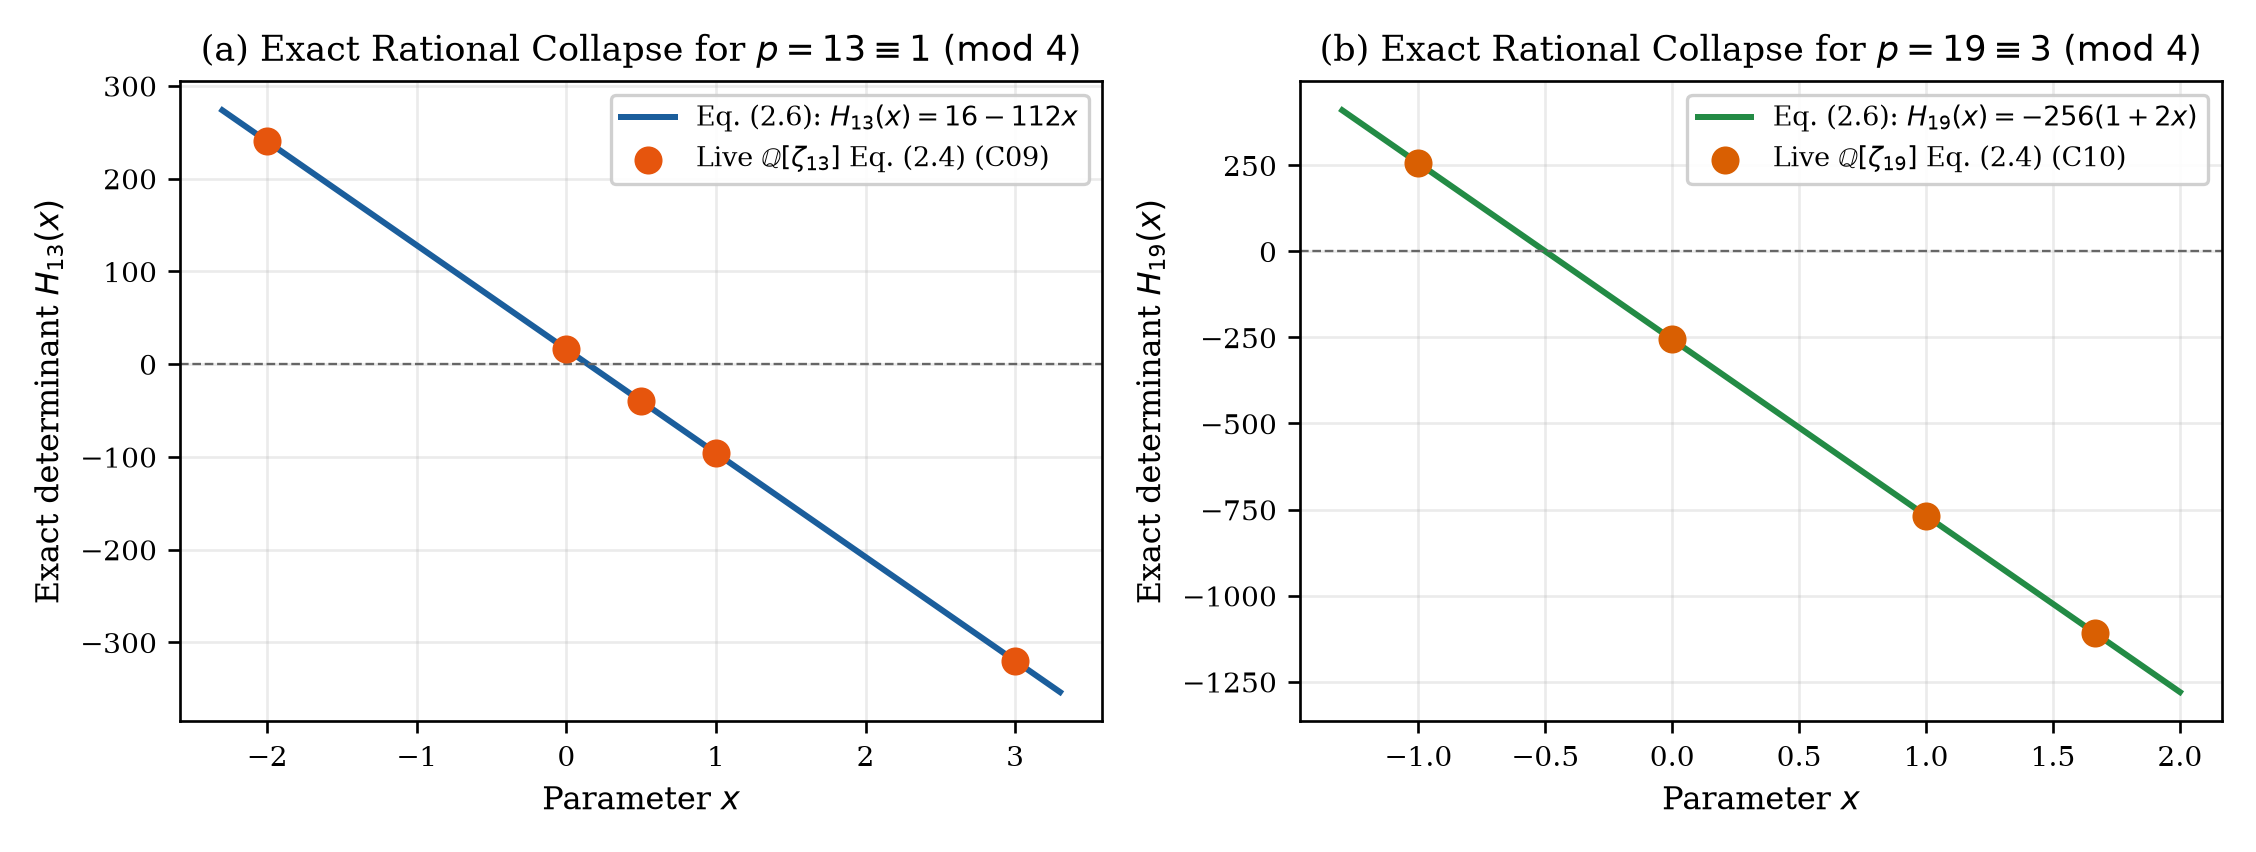
\includegraphics[width=0.90\textwidth]{figures/fig1_linear_H_collapse.png}
\caption{\textbf{Exact Cyclotomic-to-Rational Collapse (Sec.~2.6).} Evaluating Eq.~(2.4) over $\mathbb{Q}[\zeta_p]$ collapses every irrational component to zero and matches Eq.~(2.6) identically for both $p=13\equiv 1\pmod 4$ (\texttt{C09}) and $p=19\equiv 3\pmod 4$ (\texttt{C10}).}
\label{fig:fig1}
\end{figure*}

\begin{figure*}[t]
\centering
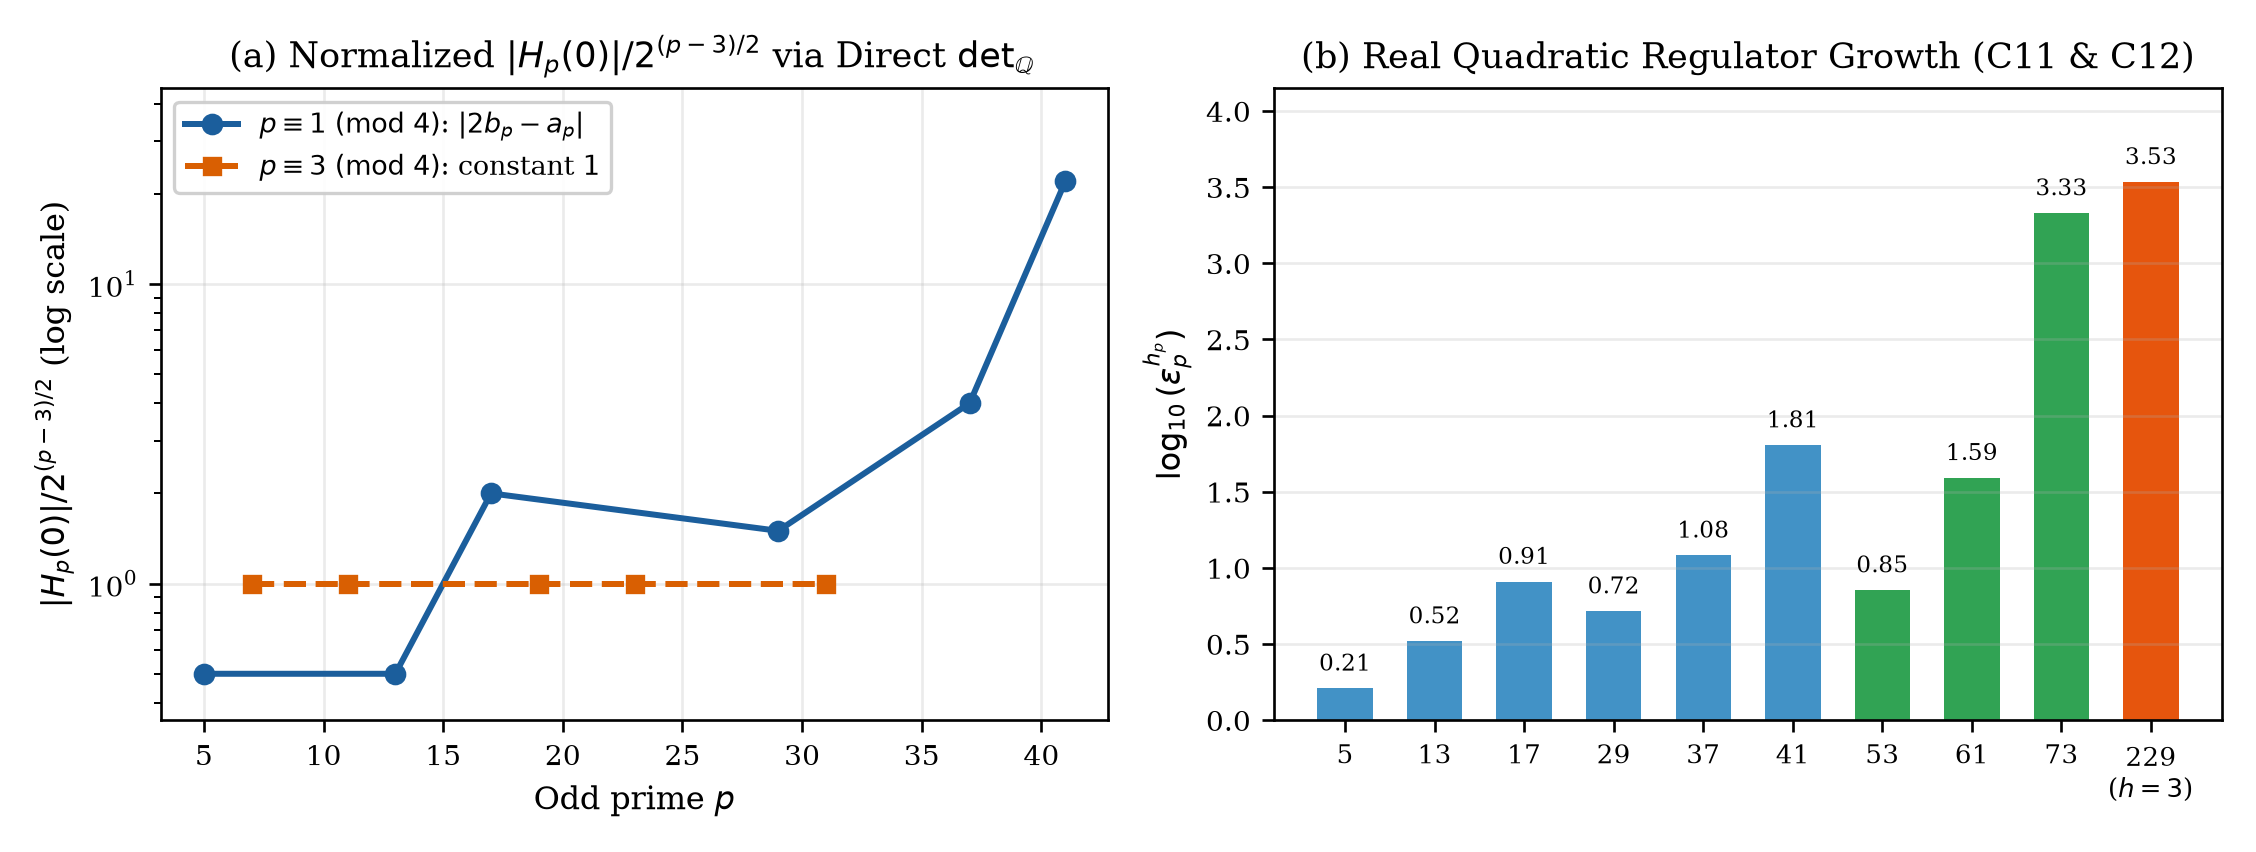
\includegraphics[width=0.90\textwidth]{figures/fig2_unit_growth_and_det_scaling.png}
\caption{\textbf{Determinant Scaling and Real Quadratic Regulators.} (a)~Normalized $|H_p(0)|/2^{(p-3)/2}$ equals $|2b_p-a_p|$ for $p\equiv 1\pmod 4$ versus constant $1$ for $p\equiv 3\pmod 4$. (b)~Logarithmic growth of $\varepsilon_p^{h_p}$ across all 10 certified primes in \texttt{C11} (blue, $p\le 41$) and \texttt{C12} (green, $h_p=1$; orange, $p=229, h_{229}=3$).}
\label{fig:fig2}
\end{figure*}

\begin{figure*}[t]
\centering
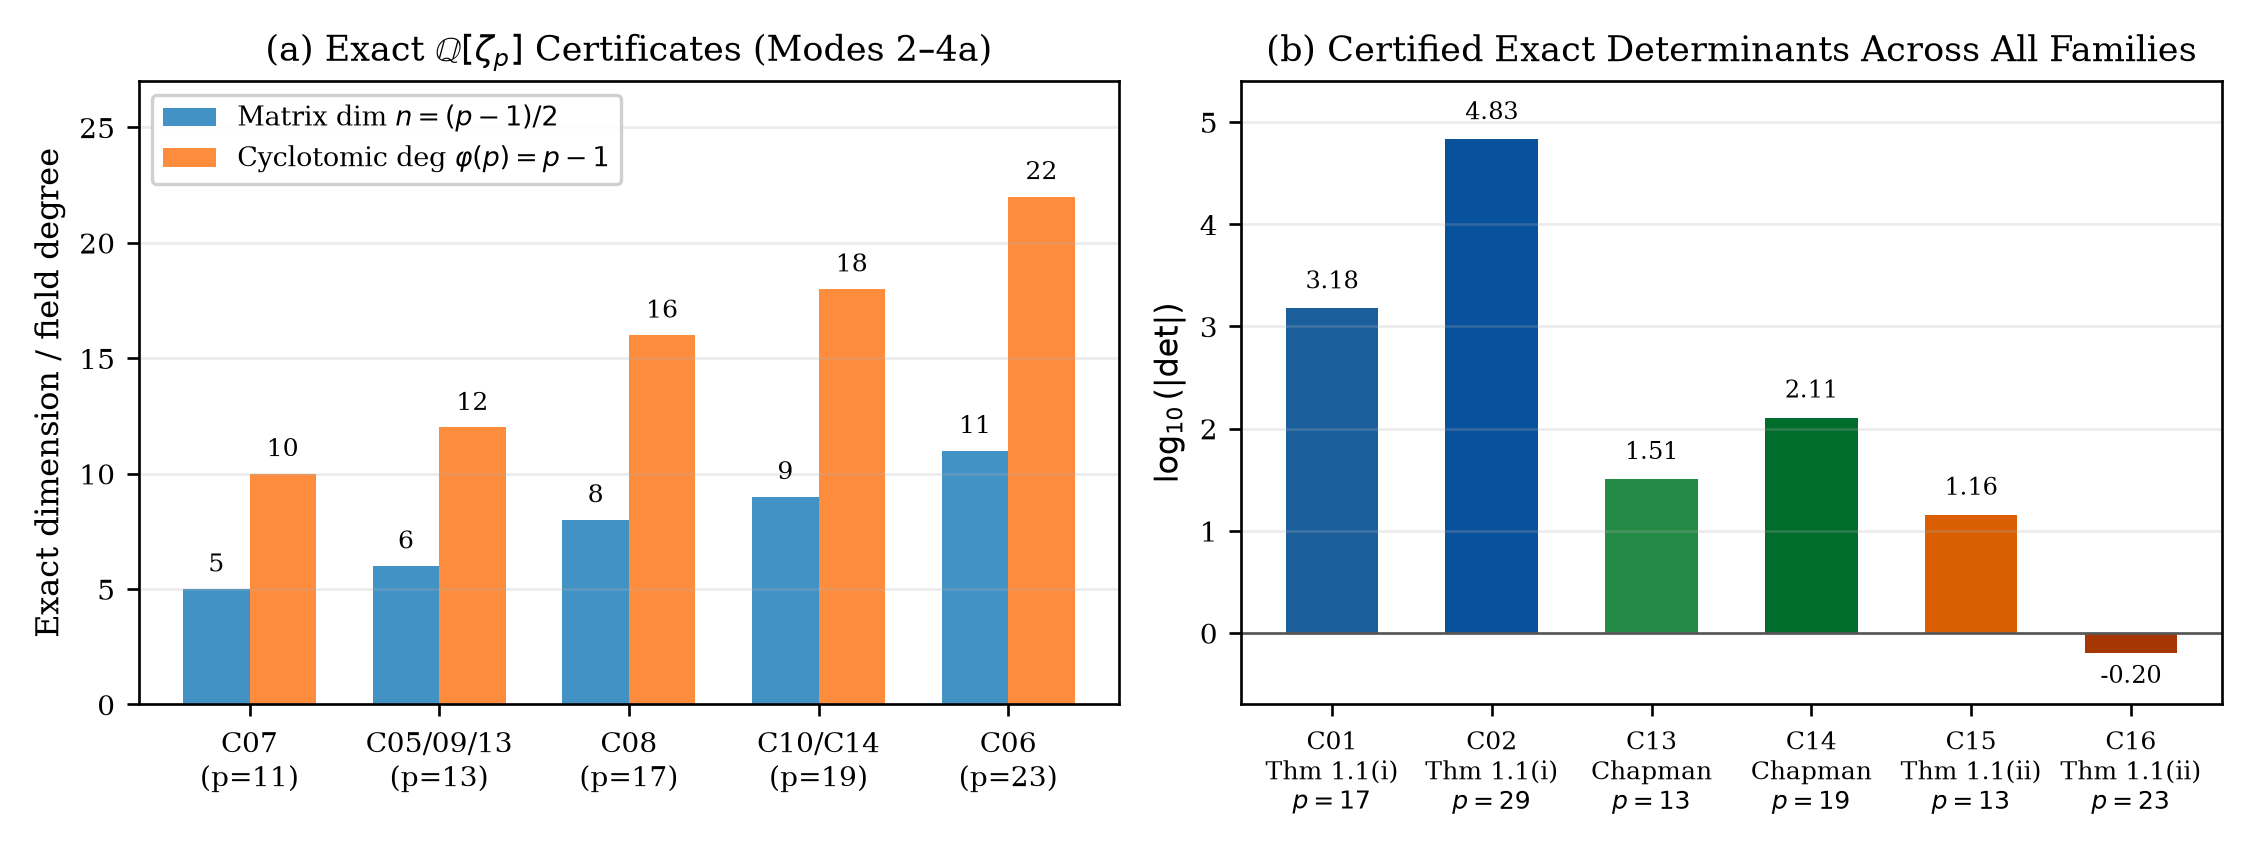
\includegraphics[width=0.90\textwidth]{figures/fig3_cyclotomic_workload_and_families.png}
\caption{\textbf{Exact $\mathbb{Q}[\zeta_p]$ Dimensions and Companion Determinant Families.} (a)~Matrix dimension $n=(p-1)/2$ and cyclotomic degree $\varphi(p)=p-1$ across live Modes~2--4a certificates. (b)~Exact logarithmic magnitudes $\log_{10}(|\det|)$ across Sun Part~(i), Chapman $F(x)$, and Sun Part~(ii).}
\label{fig:fig3}
\end{figure*}

\paragraph{Worked Witness~1 (Four-Parameter Sun Determinant at $p=17$, \texttt{C01}).}
For $p=17$ ($n=8$, $(2/17)=+1$, $2^{(p-3)/2}=128$, $\varepsilon_{17}=4+\sqrt{17}$, $h_{17}=1$), Eq.~(2.6) gives $H(0) = 128(2\cdot 1 - 4) = -256$ and $H(1) = 128((17-8) + (2-4)) = 896$. At $(x,y,z,w) = (\tfrac{3}{2}, -\tfrac{1}{3}, \tfrac{5}{4}, \tfrac{2}{5})$, we have $v = \tfrac{3}{5} - \tfrac{2}{3}\cdot\tfrac{9}{4} = -\tfrac{9}{10}$, so~\eqref{eq:thm11} predicts $128\bigl(9\cdot\tfrac{3}{2} + 2\cdot(-\tfrac{9}{10})\bigr) = 128\cdot\tfrac{117}{10} = \tfrac{7488}{5}$, matching exact $8\times 8$ Gaussian elimination over $\mathbb{Q}$ and Eq.~(2.1) identically.

\paragraph{Worked Witness~2 (Exact Cyclotomic Field Verification at $p=13$ and $p=23$, \texttt{C05}, \texttt{C06}, \texttt{C09}).}
Inside $\mathbb{Q}[\zeta_{13}]$ ($\varphi(13)=12$), Mode~2a (\texttt{C05}) confirms $\tau_{13}^2 = 13$, $c_{13} = \tfrac{13}{2} - \tfrac{3}{2}\tau_{13}$, and $\det(M)^2 = -13^2\tau_{13}(\tfrac{3}{2}+\tfrac{1}{2}\tau_{13})$, while Mode~3a (\texttt{C09}) evaluates Eq.~(2.4) at $x\in\{-2,0,\tfrac{1}{2},1,3\}$ and confirms exact collapse to $H_{13}(x) = 16 - 112x \in \{240, 16, -40, -96, -320\}$ (Fig.~\ref{fig:fig1}a). For $p=23\equiv 3\pmod 4$ (\texttt{C06}), the imaginary quadratic class number is $h_{-23}=3$, so $(-1)^{(h_{-23}+1)/2}=+1$ flips the sign in Eq.~(2.5) to $c_{23} = +\tau_{23}$ (verified in $\mathbb{Q}[\zeta_{23}]$ of degree $22$, along with $\det(M)^2 = (-23)^5 = -6{,}436{,}343$).

\paragraph{Worked Witness~3 (Higher Class Number $h_{229}=3$ and Part~(ii) Cubic Unit, \texttt{C12} \& \texttt{C15}).}
For $p=229\equiv 1\pmod 4$, $\varepsilon_{229}=\tfrac{15+\sqrt{229}}{2}$ has norm $\tfrac{225-229}{4}=-1$ and odd class number $h_{229}=3$; Mode~3b (\texttt{C12}) certifies $\varepsilon_{229}^3 = \tfrac{13680 + 904\sqrt{229}}{8} = 1710 + 113\sqrt{229}$ with exact norm $1710^2 - 229\cdot 113^2 = -1$ (Fig.~\ref{fig:fig2}b). In \texttt{C15} ($p=13$, $(2/13)=-1$), Theorem~1.1(ii) invokes $\varepsilon_{13}^3 = 18 + 5\sqrt{13}$ (Lean Theorem~16), giving $\det A_- = -18\cdot\tfrac{3}{5} + 5\cdot(-\tfrac{7}{10}) = -\tfrac{143}{10}$ matching direct $6\times 6$ exact elimination (Fig.~\ref{fig:fig3}b).

\section{Reproducibility and Availability}
All Lean~4 proofs, Python cyclotomic verifiers, certificates, figure scripts, and SHA-256 manifest (\texttt{MANIFEST.sha256}) are archived at \nolinkurl{https://github.com/lluiseriksson/legendre-symbol-determinants-certificates} under MIT (code/Lean/data) and CC-BY-4.0 (manuscript/figures) licenses. Reproduction requires three commands: \texttt{cd lean \&\& lake build}, \texttt{python -m src.legendre\_det\_verifier certificates}, and \texttt{pytest -q}.

\paragraph{AI Assistance Disclosure.}
Google Antigravity assisted with Lean~4 proof engineering, zero-float cyclotomic verifier implementation, test/figure automation, and LaTeX drafting. The author verified every mathematical derivation, Lean axiom audit, certificate check, and visual figure inspection, and takes full responsibility for all contents.

\bibliographystyle{plain}
\bibliography{references}
\end{document}
